\documentclass{article}
\usepackage[utf8]{inputenc}
\usepackage{amsmath}
\usepackage{amssymb}
\usepackage{booktabs}
\usepackage{cancel}
\usepackage{enumitem}
\usepackage{graphicx}
\usepackage{mathtools}
\usepackage{mdframed}
\usepackage{multirow}
\usepackage{pgfgantt}
\usepackage{pdflscape}
\usepackage{caption} 
\usepackage{subcaption} 
\usepackage{bbm}
\usepackage[margin=1in]{geometry}
\usepackage{biblatex} 
\addbibresource{library.bib}
\usepackage{csquotes}

\title{NE8 Lecture 5: Practical reactor physics 1, lattice physics}
\author{Paul Cosgrove}
\date{September 2022}

\begin{document}

\maketitle

We've seen the transport equation, how to simplify it, and the methods people use to solve it. But how does this help us? Ultimately our goal is to \textbf{quickly and accurately} solve reactor physics problems to estimate the power and criticality of a nuclear reactor. The modern standard for this is $\sim 1$ second for a two group\footnote{Really modern codes use six groups!} diffusion solution for a maximum of $\sim 1$\% error on all pin fission rates across a full core 3D reactor. This also accounts for thermal-hydraulics and can be used to evolve the reactor through its burn-up. Achieving this requires combining accurate nuclear data, efficient transport solutions, and fast running `nodal' diffusion methods. The next two lectures will discuss how all of these come together to give us the practical reactor physics methods used in industry.

\section{Nuclear data}

\begin{displayquote}
\textbf{Cross sections do not fall from the sky.}

\textbf{-- Eugene Shwageraus}
\end{displayquote}

If we want to accurately simulate a nuclear reactor, we need accurate nuclear data. These exist in Evaluated Nuclear Data Files (ENDFs). These files are derived from experimental data and nuclear modelling which are combined to produce the cross sections with which we are familiar. How this is done is not entirely clear to the extent that there are many different, competing nuclear data libraries -- these are often associated with different countries or different national labs. Confusingly, one of these data libraries is also called ENDF/B! The actual cross sections that these libraries contain also differ worryingly... One can easily expect a 300 pcm (0.003) difference\footnote{`pcm' is a common unit of measurement for reactivity: it stands for ``per cent mille'' and is equal to $10^{-5}$. For context, the delayed neutron fraction in LWRs is $\sim$700 pcm.} in $k_\mathrm{eff}$ produced by the same code running with different data libraries. Essentially, a lot of physics has happened even before pressing go on a transport solution. Fig.~\ref{fig:iron} is a plot from JANIS which shows the difference in the capture cross section of iron between two of the most popular libraries.

\begin{figure}[h!]
	\centering
	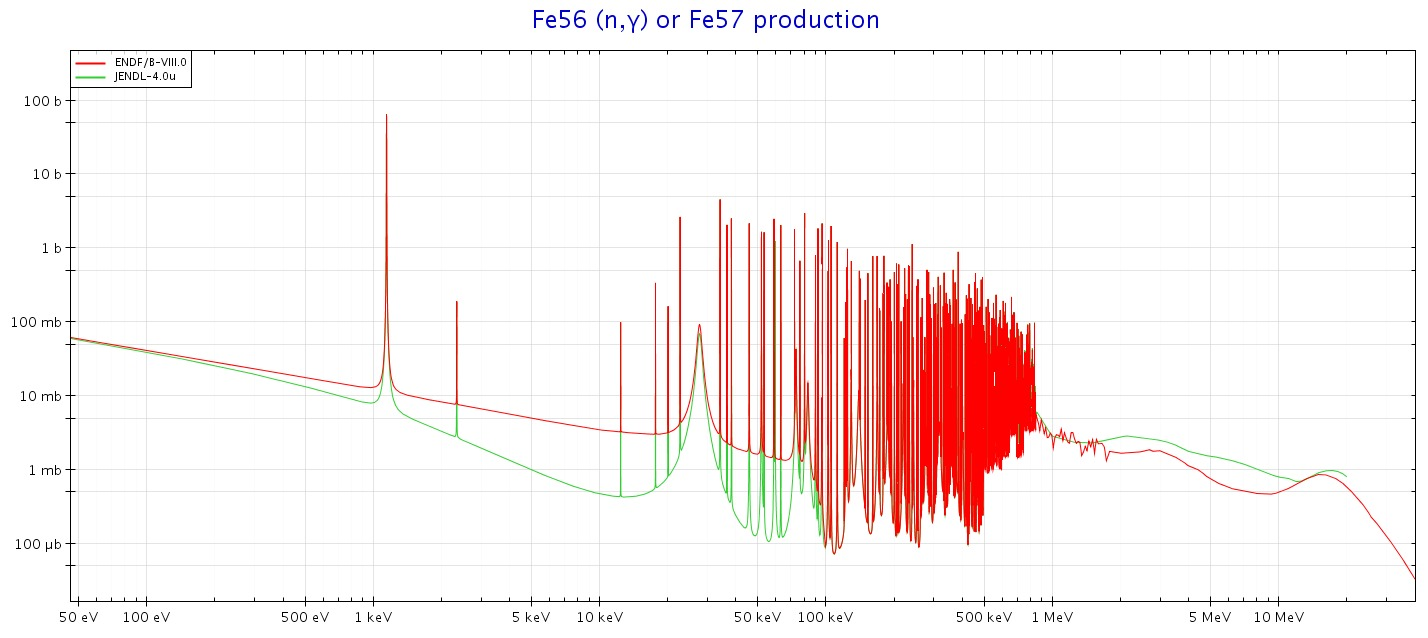
\includegraphics[scale=0.3]{./images/iron_XS.jpeg} 
	\caption{The capture cross section of iron contained in the most recent releases of the ENDF/B (U.S.) and JENDL (Japan) libraries.} 
	\label{fig:iron}
\end{figure}

\section{Multi-group cross sections}

The next difficulty is that we never solve the transport equation with continuous energy (well, unless we do Monte Carlo, but that's \textit{usually} too slow for the purposes of this lecture). We are forced to solve either the multigroup (MG) transport equation:
\begin{equation}\label{eq:mg_transport}
    \begin{split}
 \mathbf{\Omega}\cdot\nabla\psi^g + \Sigma^g_\mathrm{t}\psi^g
    =\frac{\chi^g}{4\pi k_\mathrm{eff}}\sum_{g'} \;\bar{\nu}\Sigma^{g'}_\mathrm{f}\phi^{g'} +\sum_{g'}\int_{4\pi}\mathrm{d}{\Omega}' \;\Sigma^{g'\rightarrow g}_\mathrm{s}\left(\mathbf{\Omega}'\rightarrow\mathbf{\Omega}\right)\psi^{g'}\;\mathrm{,}
    \end{split}
\end{equation}
or, when we can get away with it, the MG diffusion equation:
\begin{equation}\label{eq:mg_diffusion}
    -\nabla\cdot D^g\nabla\phi^g + \left[\Sigma^g_\mathrm{a}+\sum^G_{g'\neq g}\Sigma^{g\rightarrow g'}_\mathrm{s}\right]\phi^g = \frac{\chi^g}{k_\mathrm{eff}}\sum^G_{g'=1}\nu\Sigma^{g'}_\mathrm{f}\phi^{g'} + \sum^G_{g'\neq g} \Sigma^{g'\rightarrow g}_\mathrm{s}\phi^{g'}\;\mathrm{.}
\end{equation}
Hence, we need MG cross sections (and fission spectra and diffusion coefficients...).

What makes MG cross sections accurate? Fundamentally, we want the solutions of Eqs.~\eqref{eq:mg_transport} and \eqref{eq:mg_diffusion} to reproduce the nuclear reaction rates and criticality of a hypothetical continuous energy simulation (reality being one example). That is, for reaction $x$, occurring in the energy range $E_{g} < E\leq E_{g-1}$ we want the following to be true:
\begin{equation}
    \int^{E_{g-1}}_{E_g}\mathrm{d}E\;\Sigma_x(E)\phi(E) = \Sigma^g_x\phi^g\;\mathrm{.}
\end{equation}
When we converted the transport equation from continuous energy to MG in Lecture 1, we defined the MG flux in group $g$ as:
\begin{equation}
    \phi^g =     \int^{E_{g-1}}_{E_g}\mathrm{d}E\;\phi(E)\;\mathrm{,}
\end{equation}
and therefore our MG cross section can be written as:
\begin{equation}\label{eq:MG}
    \Sigma^g_x = \frac{\int^{E_{g-1}}_{E_g}\mathrm{d}E\;\Sigma_x(E)\phi(E)}{\int^{E_{g-1}}_{E_g}\mathrm{d}E\;\phi(E)}\;\mathrm{.}
\end{equation}
In other words, a MG cross section is a spectrum-averaged (or flux-weighted average) cross section in the given energy range. This definition of a MG cross section ensures that \textbf{reaction rates are preserved}. In principle we could define our MG cross sections in other ways, e.g., as a simple energy-averaged cross section, but this wouldn't be very accurate unless we used many small energy groups. The important thing to know is that \textbf{the more coarsely we want to discretise energy, the better we need to know the spectrum}.

Note, while I have used macroscopic cross sections in the equations here, all of these considerations apply equally to microscopic cross sections -- this will be especially important when we consider isotopic depletion!

\section{Producing multi-group cross sections}

\begin{displayquote}
\textbf{``Wait a minute,'' you ask, ``the purpose of solving the transport equation is to get the flux, but I have to know the flux to compute the multi-group constants!''}

\textbf{-- The NJOY manual}
\end{displayquote}

The most difficult aspect of deterministic neutronics in reactors is generating accurate cross sections because creating `good' cross sections requires already knowing the spectrum. We could avoid this if we solved a $\sim$100s of groups high-fidelity transport problem across a whole core immediately, but that has (until recently) been inconceivable due to computer time and memory constraints. It would also have to be solved many times to account for changes in temperature, boron, and burn-up.

Historical computational constraints have resulted in reactor physicists generating cross sections in several stages, applying different approximations and discretisations and accounting for different space and energy effects at each stage. This is the domain of \textbf{lattice physics codes}. `Lattice' refers to a fuel pin or an assembly in an infinite lattice, the logic being that cross sections are mostly determined by the local conditions which assemblies see, rather than by their relative position in a reactor core. These codes aim to generate spatially-homogenised few-group cross sections in each assembly that features in a reactor core, subject to all operating conditions it will see (changes in fuel temperature, moderator density, burn-up...). WIMS\footnote{WIMS stands for Winfrith Improved Multigroup Scheme.} (which you will use for the coursework) was the first of these codes, but many more now exist and are used throughout industry. CASMO\footnote{I don't think CASMO stands for anything.} is arguably the most famous lattice physics tool due to its speed, accuracy, and user-friendliness. Most of these tools also have a partner nodal diffusion code -- the fast running coarse mesh diffusion code which uses all of these cross sections to quickly solve whole core reactor problems, including feedbacks from other physics. This will be discussed next lecture.

The process of generating many accurate MG cross sections starts from NJOY or an equivalent. NJOY\footnote{NJOY doesn't stand for anything: it's a one-letter shift of it's predecessor, MINX.} is a nuclear data processing code developed at Los Alamos that translates pointwise-in-energy ENDF files into fine-group cross section data as an input for neutronics codes. To do this, NJOY begins by making an educated guess as to what the spectrum looks like in certain energy ranges.

For fast neutrons (1 MeV $< E <$ 20 MeV) the spectrum is often well characterised by the uranium fission spectrum, $\chi(E)$, as that is the dominant source. For intermediate range neutrons ($\sim$1 eV $< E <$ 1 MeV), where slowing down and scattering is dominant, the spectrum can be approximated as a $1/E$ shape (we'll try and justify this shortly). Finally, at thermal energies where neutrons begin to upscatter ($E < $ 1 eV), the spectrum can be approximated with a Maxwell-Boltzmann distribution. 

Of course this is not entirely true: in all of these regions, resonances and spatial effects can greatly perturb these spectra, but it's a starting point for the production of fine-group cross sections. One of the main functions of any lattice physics code is to apply `resonance treatment', i.e., account for the effects of resonances in the problem of interest on the cross sections so that reaction rates are appropriately preserved.

There is \textbf{a lot} of physics that goes into producing cross sections. There is even more maths and none of that is very interesting to go through in a lecture. Instead, I'm going to tell you which approximations we make and I'll do my best to justify them where they can be justified. I don't expect anyone to know or remember all of this -- my main hope is that if you ever happen to be using a lattice physics tool more seriously in the future then this will be a good place to start. But there might be a few more relevant bits for NE8 along the way!

The following discussion closely follows (and greatly abridges) Knott \& Yamamoto~\cite{Knott}.

\section{Neutron slowing down}

\subsection{Slowing down in hydrogen}
It is stated above that at intermediate energies the spectrum is given by $\phi(E) \propto 1/E$. Is this a good approximation? This is said to be valid where there is little absorption, no strong sources, and no upscattering, i.e., in energy ranges away from where fission neutrons are produced, above thermal energies, and away from absorbers. You might be worried that hydrogen is an absorber, but it is a much stronger scatterer ($\frac{\sigma_\mathrm{a,H}}{\sigma_\mathrm{s,H}}\sim 0.014$). We need to assume there aren't many resonances around -- which is certainly true for a hydrogen moderator. For faster neutrons, mean free paths are also longer due to lower cross sections, making the geometry appear more homogeneous.

How can this be derived? Assume we are in an infinite homogeneous medium: the transport equation will lose the $\mathbf{\Omega}\cdot\nabla \psi$ term and we can integrate over all directions to express the equation in terms of scalar flux alone. We will refer only to scattering and some other generic source of neutrons, $S_0$ producing neutrons at energy $E_0$ which is the highest energy source in the problem. If we also say that we are sufficiently energetic so that neutrons can only downscatter, we have:
\begin{equation}\label{eq:slowing_down}
    \Sigma_\mathrm{t}(E)\phi(E) = \int^{E_0}_E \mathrm{d}E'\;\Sigma_\mathrm{s}(E'\rightarrow E)\phi(E') + S_0\delta(E-E_0)\;\mathrm{.}
\end{equation}
First, there is no absorption, so $\Sigma_\mathrm{t}(E)\rightarrow \Sigma_\mathrm{s}(E)$. If most of the scattering is elastic scattering on hydrogen then we can write:
\begin{equation}
    \Sigma_\mathrm{s}(E'\rightarrow E) = \begin{cases}
    \frac{\Sigma_\mathrm{s}(E')}{(1-\alpha)E'},& \text{if } E<E'<\frac{E}{\alpha}\\
    0,              & \text{otherwise}
\end{cases}
\end{equation}
You may recall this from NE1, where $\alpha = \left(\frac{A-1}{A+1}\right)^2$ and $A$ is the atomic mass ratio of the scattering atom to the neutron. We also assume that the scattering cross section is constant. This may seem like a big leap, but it is often true for common moderators. This is because potential scattering is dominant in this region -- here the cross section is determined by the nuclear radius (which is independent of neutron energy). This can be seen in Fig.~\ref{fig:hydrogen_scatter} for hydrogen. 

\begin{figure}[h!]
	\centering
	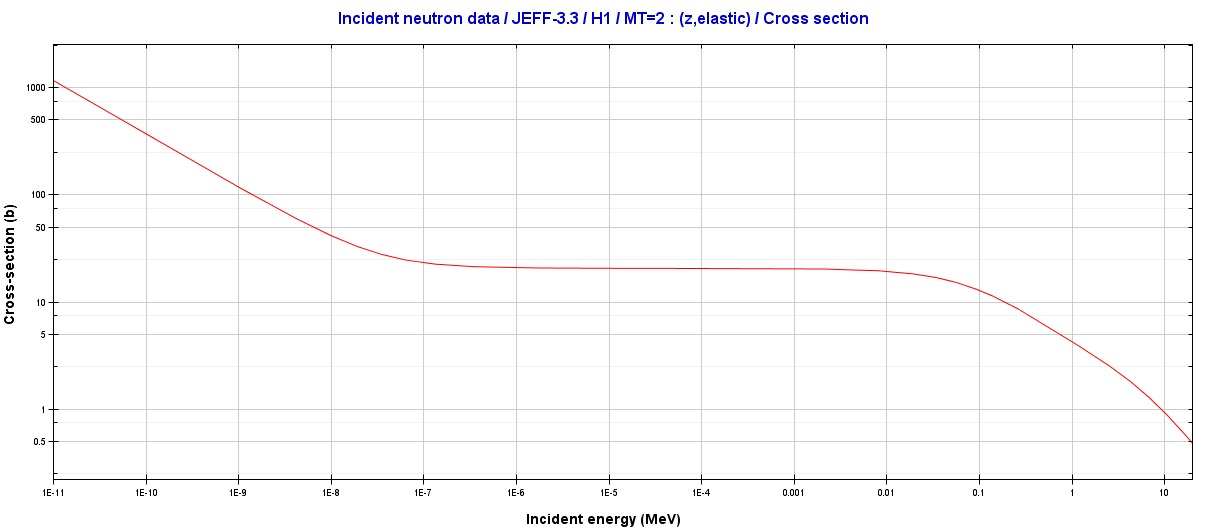
\includegraphics[scale=0.3]{./images/hydrogen_XS.jpeg} 
	\caption{The scattering cross section of hydrogen -- note the flat region in the middle where potential scattering is dominant.} 
	\label{fig:hydrogen_scatter}
\end{figure}

Combining all of this together and using some integral equation tricks ultimately gives:
\begin{equation}
    \phi(E) = \frac{S_0}{\Sigma_\mathrm{s}E} + \frac{S_0}{\Sigma_\mathrm{s}}\delta(E-E_0)\;\mathrm{.}
\end{equation}
What this equation says is that our flux is proportional to $1/E$ at energies far away from the source. Furthermore, the stronger the source, the greater the proportionality constant (intuitively enough). Much more detail can be found on this between pages 317-321 of Duderstadt \& Hamilton \cite{Duderstadt}. The $1/E$ spectrum is often referred to as \textbf{the asymptotic spectrum}.

How does this compare against reality? Using the Serpent Monte Carlo code (essentially an exact physics treatment), I made a box full of only water with reflective boundaries (so an infinite medium) and put a point source of neutrons at 2 MeV in the middle. The spectrum is shown in Fig.~\ref{fig:1_E}. As you can see, the fit is actually pretty good!

\begin{figure}[h!]
	\centering
	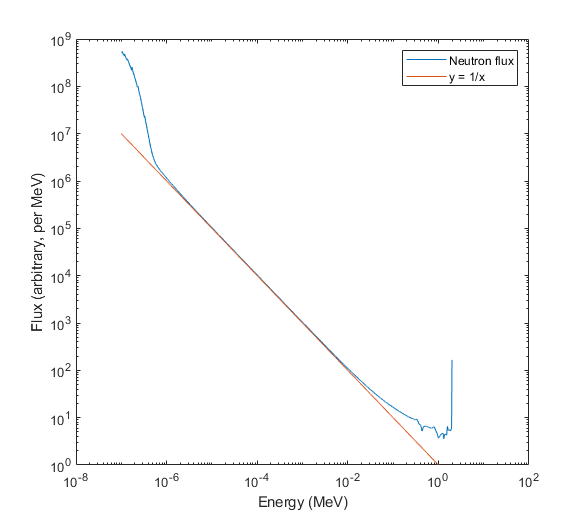
\includegraphics[scale=0.9]{./images/asymptotic_flux.png} 
	\caption{The spectrum produced by neutrons slowing down in water without any absorbers. The jaggedness around 1 MeV is due to the beginning of oxygen's resonance range.} 
	\label{fig:1_E}
\end{figure}

\subsection{Slowing down with resonant absorbers}

But this is extremely simple. The main problem we want to address is how this spectrum changes in the presence of resonant absorbers. We need to make more approximations to do this. For now we will assume there is a resonant nuclide denoted by $r$ and other non-resonant nuclides denoted by $k$. We will assume no energy dependence for the cross sections of non-resonant nuclides and they have no absorption, i.e., only potential scattering occurs. This is a justifiable assumption in the resonance energy range. Therefore our slowing down equation becomes:
\begin{equation}\label{eq:full_slowing_down}
    \left(N_r\sigma_{\mathrm{t},r}+\sum_{k\neq r}N_k\sigma_{\mathrm{p},k}\right)\phi(E) = \int^{E/\alpha_r}_E \frac{N_r \sigma_{\mathrm{s},r}(E')}{1-\alpha_r}\phi(E')\frac{\mathrm{d}E'}{E'} + \sum_{k\neq r}\int^{E/\alpha_k}_E \frac{N_k \sigma_{\mathrm{p},k}}{1-\alpha_k}\phi(E')\frac{\mathrm{d}E'}{E'}\;\mathrm{.}
\end{equation}
Here we have separated the macroscopic cross sections into their microscopic cross section and the nuclide density, $N$. Unfortunately this equation remains very complicated to solve and so still more assumptions are necessary!

We can simplify things by assuming that resonances are \textbf{narrow compared to the slowing down width} (neutrons lose much more energy in a collision than the width of the resonance). As a result, away from the resonance the $1/E$ spectrum holds. This also implies the resonance's contribution to the integration is small because of its narrow width. With these approximations, the non-resonant term in Eq.~\eqref{eq:full_slowing_down} becomes, simply $\sum_{k\neq r}N_k\sigma_{\mathrm{p},k}/E$ (letting the source proportionality constant just equal 1).

If we also assume that the scattering part of the resonant nuclide is also constant in energy and that the spectrum shape is \textit{approximately} $1/E$ then for the resonant portion of the RHS of Eq.~\eqref{eq:full_slowing_down} we get $N_r\sigma_{\mathrm{p},r}/E$.

Putting this together and getting the flux by itself gives the approximate spectrum subject to the \textbf{narrow resonance approximation}:
\begin{equation}\label{eq:NR}
    \phi(E) = \frac{N_r\sigma_{\mathrm{p},r}+\sum_{k\neq r}N_k\sigma_{\mathrm{p},k}}{N_r\sigma_{\mathrm{t},r}(E) + \sum_{k\neq r}N_k\sigma_{\mathrm{p},k}}\frac{1}{E} = \frac{\sigma_{\mathrm{p},r}+\sigma_0}{\sigma_{\mathrm{t},r}(E) + \sigma_{0}}\frac{1}{E}\;\mathrm{,}
\end{equation}
where we have defined the \textbf{background cross section}, $\sigma_0$, as:
\begin{equation}
    \sigma_0 = \frac{\sum_{k\neq r}N_k\sigma_{\mathrm{p},k}}{N_r}\;\mathrm{.}
\end{equation}
This is a fictitious cross section which describes the relative importance of scattering away from the resonance to resonance absorption. When it is small, the flux shape is greatly perturbed by the resonance -- this corresponds to the resonant absorber having a relatively high concentration. On the other hand, when the background cross section is large, the flux is not perturbed by the absorber and returns to having the $1/E$ shape -- the absorber does not matter or is extremely `dilute'.

How does this compare against reality? I put some $^{238}$U into the watery box above at various different concentrations. Running a few Serpent calculations, the resulting spectra are plotted in Fig.~\ref{fig:dilution}. Knowing the densities of each isotope, the potential scattering cross sections of hydrogen and oxygen, and a rough guess at the potential cross section of 238, I was able to calculate the background cross section for each case. Then, I used Eq.~\eqref{eq:NR} to obtain some spectra assuming the narrow resonance approximation. These are shown in Fig.~\ref{fig:NR}. 

There are a few differences: first, the magnitude of the Serpent spectra for low dilutions decreases due to neutron absorption whereas the NR spectra return to the $1/E$ magnitude. This is because neutrons in the Serpent calculation are actually being absorbed. However, this isn't a very big deal, because we only care about the shape of the spectra, not the absolute magnitude. We also note that the Serpent spectra have `jumps'. This is due to the resonant scattering cross section of $^{238}$U which the NR approximation explicitly fails to account for. Thankfully, these are fairly small and isolated.

\begin{figure}[h!]
	\centering
	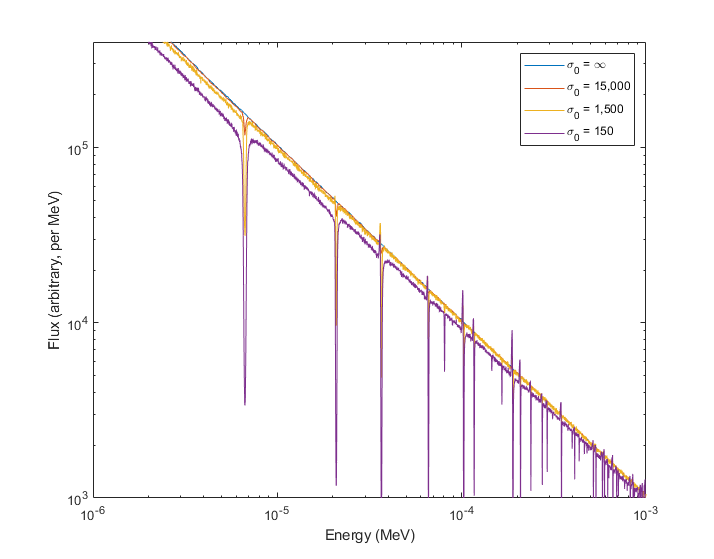
\includegraphics[scale=0.6]{./images/dilution_238.png} 
	\caption{The spectra produced by neutrons slowing down in water with various concentrations of $^{238}$U.} 
	\label{fig:dilution}
\end{figure}

\begin{figure}[h!]
	\centering
	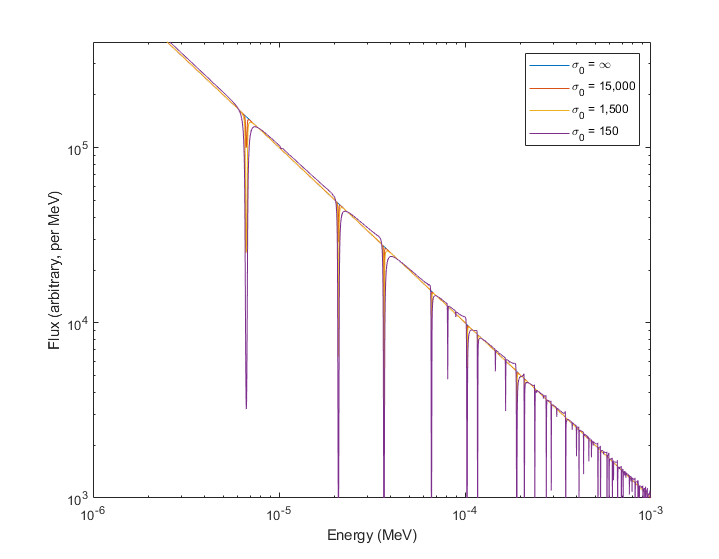
\includegraphics[scale=0.6]{./images/NR_238.png} 
	\caption{The spectra produced by the narrow resonance approximation with various background cross sections of $^{238}$U.} 
	\label{fig:NR}
\end{figure}

While many resonances are indeed narrow (particularly at higher energies), some are very wide with respect to the neutron slowing down width, e.g., $^{238}$U's largest resonance about 6.67 eV. This renders Eq.~\eqref{eq:NR} even more inaccurate. Thus we often use the \textbf{wide resonance approximation} as well. The basis of the approximation is that the resonant nuclide has infinite mass, so neutrons lose no energy on collision with it. This gives a slightly different form for the flux:
\begin{equation}\label{eq:WR}
    \phi(E) =  \frac{\sigma_0}{\sigma_{\mathrm{a},r}(E) + \sigma_{0}}\frac{1}{E}\;\mathrm{.}
\end{equation}
This amounts to neglecting the scattering component of the resonant nuclide. This is plotted as well for $^{238}$U in Fig.~\ref{fig:WR}. This does a noticeably better job of capturing the flux perturbation caused by low energy resonances.

\begin{figure}[h!]
	\centering
	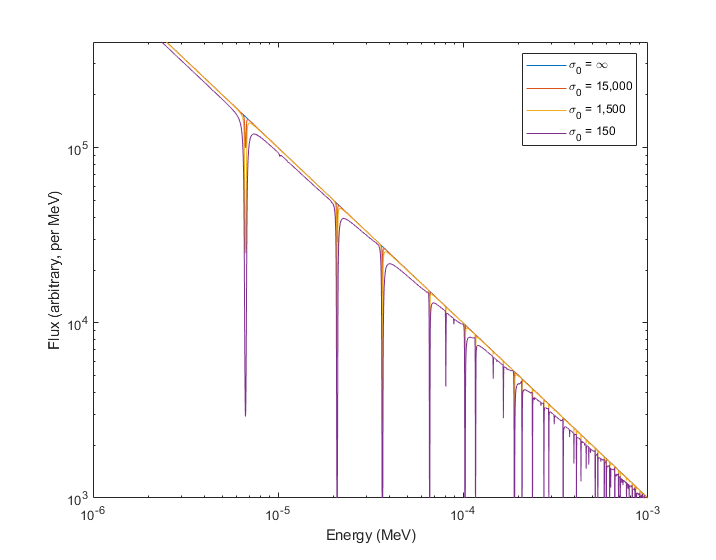
\includegraphics[scale=0.6]{./images/WR_238.png} 
	\caption{The spectra produced by the wide resonance approximation with various background cross sections of $^{238}$U.} 
	\label{fig:WR}
\end{figure}

When generating multi-group cross sections, these equations are used to handle the energy self-shielding effect \textbf{in homogeneous mixtures}. Most nuclear reactors, on the other hand, are heterogeneous. This can also lead to flux perturbations which must be accounted for.

\subsection{Accounting for heterogeneity}

Most reactor systems are heterogeneous and this will also result in perturbations to the asymptotic spectrum, thus affecting the multi-group cross sections we would obtain.

The standard way to analyse this is to begin by saying we are in an \textbf{isolated system}: we have a lump of (resonant) fuel sitting in an infinite sea of moderator. This is obviously unrealistic, but we'll fix that later!

Historically we didn't want to use sophisticated (expensive) means of accounting for the spatial dependence of the flux. Instead, we used the collision probabilities formalism for a simple two-region problem. We consider the collision rate in our fuel, accounting for neutrons which appear in the fuel and collide in the fuel and neutrons which appear in the moderator and collide in the fuel:
\begin{equation}\label{eq:multiregion_slowing_down}
    \Sigma_{\mathrm{t,f}}(E)\phi_\mathrm{f}(E)V_\mathrm{f} = P_{\mathrm{f}\rightarrow\mathrm{f}}(E)V_\mathrm{f}\int^{\infty}_0\mathrm{d}E'\;\Sigma_\mathrm{s,f}(E'\rightarrow E)\phi_\mathrm{f}(E') + P_{\mathrm{m}\rightarrow\mathrm{f}}(E)V_\mathrm{m}\int^{\infty}_0\mathrm{d}E'\;\Sigma_\mathrm{s,m}(E'\rightarrow E)\phi_\mathrm{m}(E')\;\mathrm{,}
\end{equation}
where f denotes a property of the fuel, m denotes a property of the moderator, $P_{x \rightarrow y}$ is a collision probability going from region $x$ to region $y$ and $V$ is the volume of a given region. Generally speaking, collision probabilities are hard to calculate. However, in keeping with the theme, lattice physics codes make some approximations to make things quick and easy!

First, we're going to apply the approximations we made before: elastic scattering and the narrow resonance approximation transform Eq.~\eqref{eq:multiregion_slowing_down} into:
\begin{equation}
     \Sigma_{\mathrm{t,f}}(E)\phi_\mathrm{f}(E)V_\mathrm{f} = \frac{1}{E}\left(P_{\mathrm{f}\rightarrow\mathrm{f}}(E)V_\mathrm{f}\Sigma_\mathrm{p,f} + P_{\mathrm{m}\rightarrow\mathrm{f}}\Sigma_\mathrm{p,m}(E)V_\mathrm{m}\right)\;\mathrm{.}
\end{equation}

Having multiple different collision probabilities complicates things: we would rather have just one that we can calculate/approximate. We do this by using a few properties of collision probabilities.

First, probabilities must sum to 1. Therefore, when there are only two regions,the fuel-to-fuel collision probability can be rewritten in terms of the fuel-to-moderator collision probability:
\begin{equation}
    P_{\mathrm{f}\rightarrow\mathrm{f}}(E) = 1 - P_{\mathrm{f}\rightarrow\mathrm{m}}(E)\;\mathrm{.}
\end{equation}

Second, we can use what is known as the \textbf{reciprocity theorem} for collision probabilities. This simply states that:
\begin{equation}
    P_{\mathrm{f}\rightarrow\mathrm{m}}(E)V_\mathrm{f}\Sigma_{\mathrm{t,f}}(E) = P_{\mathrm{m}\rightarrow\mathrm{f}}(E)V_\mathrm{m}\Sigma_{\mathrm{t,m}}(E)\;\mathrm{.}
\end{equation}
The logic of this theorem is that the attenuation that neutrons experience is independent of direction: going from A to B will give the same amount of neutron attenuation as going from B to A. The volume and cross section factor are then used to rescale the probabilities back into attenuation factors, giving the equivalence.

Combining these two features, we finally get:
\begin{equation}\label{eq:f_to_m}
    \phi_\mathrm{f}(E) = \frac{1}{E}\left(\left(1-P_{\mathrm{f}\rightarrow\mathrm{m}}(E)\right)\frac{\Sigma_{\mathrm{p,f}}}{\Sigma_{\mathrm{t,f}}(E)} + P_{\mathrm{f}\rightarrow\mathrm{m}}(E)\right)\;\mathrm{.}
\end{equation}
The only remaining problem is to work out what $P_{\mathrm{f}\rightarrow\mathrm{m}}(E)$ is. Sadly, this is not trivial -- generally speaking it would require either using a very specific geometry or lots of ray tracing which would be too expensive. Thus we will do what we usually do and make another approximation.

$P_{\mathrm{f}\rightarrow\mathrm{m}}(E)$ is also known as the \textbf{escape probability}, $P_\mathrm{e}(E)$, literally the probability that a neutron born in the fuel escapes. The actual definition of this is:
\begin{equation}\label{eq:escape}
    P_\mathrm{e}(E) = \frac{1}{4\pi\Sigma_\mathrm{t,f}(E)V_\mathrm{f}}\int_{\mathbf{n}\cdot\mathbf{\Omega}>0}\mathrm{d}\Omega \int_S \mathrm{d}S (\mathbf{n}\cdot\mathbf{\Omega})\left(1-\exp\left(-\Sigma_\mathrm{t,f}(E)l\right)\right)\;\mathrm{,}
\end{equation}
where $S$ is the surface enclosing the fuel and $\mathbf{n}$ is the normal vector from the surface at a given point, and $l$ is the distance from a neutron's position to the surface when travelling in direction $\mathbf{\Omega}$, also known as the `chord length'. This account for all paths neutrons can take to leak out of fuel, including the attenuation that they may suffer along the way. Making something simple out of this would take knowing how the chord length is distributed across all different points in the fuel, whatever its shape may be. As usual, we make an assumption! If we assume the chord length has an exponential distribution then Eq.~\eqref{eq:escape} becomes simply:
\begin{equation}\label{eq:wigner}
     P_\mathrm{e}(E) = \frac{1}{\Sigma_\mathrm{t,f}(E)\Bar{l} + 1}\;\mathrm{,}
\end{equation}
where $\Bar{l}$ is the assumed average chord length. This is known as Wigner's Rational Approximation. This equation is very rational in the limits: if the fuel is very optically thin, then $\Sigma_\mathrm{t,f}(E)\Bar{l}\rightarrow 0$, and therefore $P_\mathrm{e}(E)\rightarrow 1$. Likewise, for optically thick fuel, $\Sigma_\mathrm{t,f}(E)\Bar{l}\rightarrow \infty$, $P_\mathrm{e}(E)\rightarrow 0$. Sadly, this isn't a very good assumption, but we use it anyway with some corrections because it has a nice feature...

As an aside, most lattice physics codes do try to correct the rational approximation. This is done in two ways:
\begin{enumerate}
    \item The Bell factor: this is an empirical number which corrects the bad approximation of the chord length distribution directly. The Bell factor, $a$, tends to be between 1.1-1.4 in LWRs and modifies the escape probability as $P_\mathrm{e}(E) = \frac{1}{1+\Sigma_\mathrm{t,f}(E)\Bar{l}/a}$. While this improves accuracy in the intermediate optical chord length range where reactor fuel designs tend to exist, it induces a 10\%-40\% bias in the escape probability for optically thick problems.
    \item The Dancoff factor: we began by assuming that fuel is isolated, surrounded by infinite moderator. This is obviously wrong. While a neutron may escape fuel, there is a chance that it won't collide with the moderator and will collide with some other fuel in the reactor. The Dancoff factor corrects this assumption by accounting for some portion of escaping neutrons colliding in or being `shadowed' by other fuel.
\end{enumerate}

\subsection{Equivalence theory}

We are able to use everything we have done so far to derive an ``equivalence'' between heterogeneous problems and homogeneous problems.

We can rewrite Eq.~\eqref{eq:f_to_m} as:
\begin{equation}
    \phi_\mathrm{f}(E) = \frac{1}{E}\left(\left(1-P_{\mathrm{e}}(E)\right)\frac{\Sigma_{\mathrm{p,f}}}{\Sigma_{\mathrm{t,f}}(E)} + P_{\mathrm{e}}(E)\right)\;\mathrm{.}
\end{equation}
If we insert Eq.~\eqref{eq:wigner} for $P_\mathrm{e}(E)$ we obtain the following after a little bit of algebra:
\begin{equation}
    \phi_\mathrm{f}(E) = \frac{1}{E}\frac{\Sigma_\mathrm{p,f}+1/\Bar{l}}{\Sigma_\mathrm{t,f}(E)+1/\Bar{l}}\;\mathrm{.}
\end{equation}
If we define an \textbf{escape cross section} as $\Sigma_\mathrm{e} = 1/\Bar{l}$ then this equation can be written as:
\begin{equation}
    \phi_\mathrm{f}(E) = \frac{1}{E}\frac{\Sigma_\mathrm{p,f}+\Sigma_\mathrm{e}}{\Sigma_\mathrm{t,f}(E) + \Sigma_\mathrm{e}} = \frac{1}{E}\frac{N_r(\sigma_\mathrm{p,r}+\sigma_{0,\mathrm{f}})+\Sigma_\mathrm{e}}{N_r(\sigma_\mathrm{t,r}(E)+\sigma_{0,\mathrm{f}})+\Sigma_\mathrm{e}}=\frac{1}{E}\frac{\sigma_{\mathrm{p},r}+(\sigma_{0,\mathrm{f}}+\Sigma_\mathrm{e}/N_r)}{\sigma_{\mathrm{t},r}(E)+(\sigma_{0,\mathrm{f}}+\Sigma_\mathrm{e}/N_r)}\;\mathrm{.}
\end{equation}
Why is this interesting? If we compare this equation with Eq.~\eqref{eq:NR} then there is a remarkable similarity. They differ only in the addition of the escape cross section to the top and bottom. As such, the escape cross section and the background cross section serve exactly the same purpose! Having a low background cross section is the same as having a low escape cross section and vice versa: the former circumstance means the asymptotic flux will be greatly perturbed, while the latter means it will be unperturbed. 

Therefore, codes like NJOY need not know about the heterogeneity to which a given nuclide cross section is subjected. If they produce cross sections at a variety of different background cross sections, they are equally valid whether the system is homogeneous or heterogenous!

\subsection{Practical implications}

Given all of this, how calculations proceed is as follows:

\begin{enumerate}
    \item Nuclear data exists in the form of nuclear data libraries in the form of ENDFs.
    \item We ask NJOY to produce fine-group cross sections in the library format of our particular lattice physics code. This will be done for all nuclides of interest to our calculation and at all \textbf{temperatures} relevant to our calculation (to include Doppler broadening).
    \item NJOY assumes a Maxwellian spectrum in the thermal range, a fission spectrum in the fast range, and either Eqs.~\eqref{eq:NR} or \eqref{eq:WR} in the intermediate range to generate multi-group cross sections using Eq.~\eqref{eq:MG}. For all nuclides, it produces a tabulation of cross sections, depending on the temperature range and the range of background cross sections requested. This is because the background cross section to which a nuclide will be subjected isn't known upfront (and can even vary over time due to burn-up).
    \item With this data and the material and geometry input to the code, a lattice physics code is able to determine what the temperature and actual background cross section is for each nuclide (by calculating the escape probability and considering all nuclides present in the problem relative to a given resonant nuclide) and so selects or interpolates the appropriate cross section set to use from the NJOY data.
\end{enumerate}

Along the way, as we have seen, many approximations were made. However, for LWRs, this approach has proved very successful in producing data of acceptable accuracy for reactor core design. Admittedly, newer approaches are used by many codes (such as the sub-group method or direct solution of the slowing down equations), but they are beyond the scope of this course. They are also more accurate, but more expensive. For example, Equivalence Theory does not account for the overlap of resonances; while this effect may not be significant for fresh UO$_2$ fuel, if the fuel has significant burn-up (and so lots of resonant fission products or actinides) or contains MOX then this may induce substantial errors!

Equivalence theory also does not work very well in either the fast or thermal regions. As such, resonances in these regions can pose problems for accuracy. Fig.~\ref{fig:WIMS} shows the classic WIMS 69 group structure and its energy discretisation. As you can see, many of the groups are focused on the low-lying plutonium resonances which would be hard to accurately treat with equivalence theory but which dictate much of reactor physics after just a bit of burn-up.

\begin{figure}[h!]
	\centering
	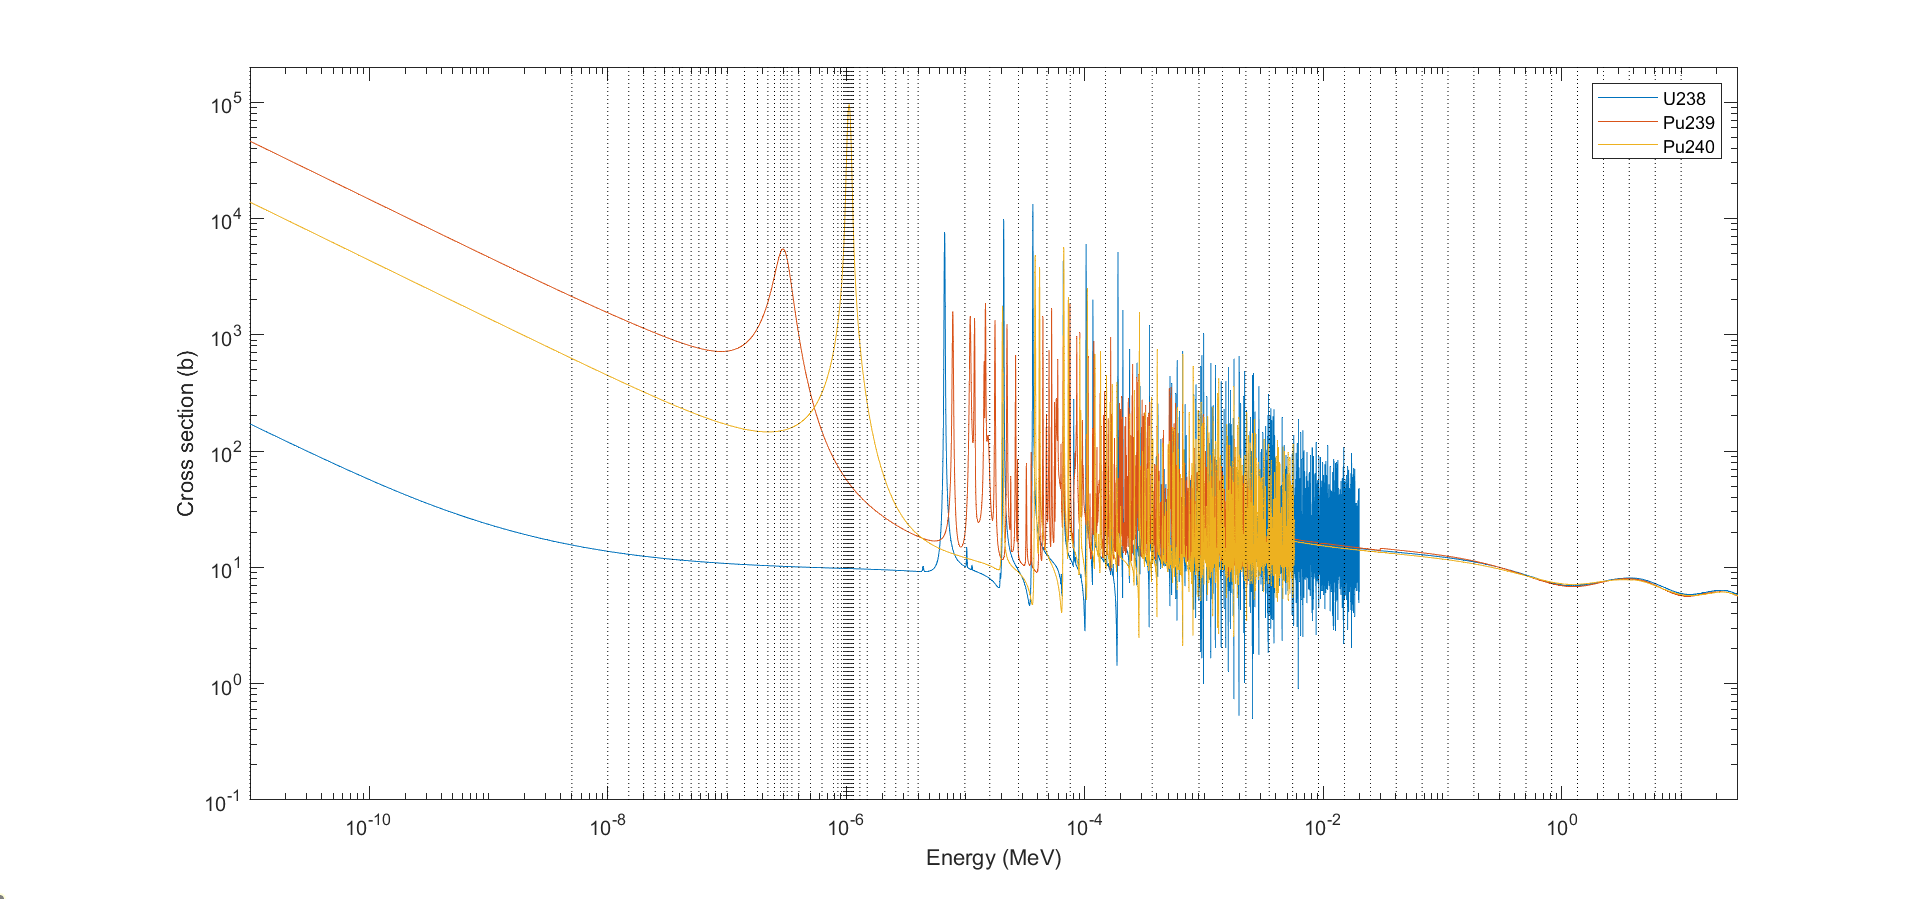
\includegraphics[scale=0.3]{./images/cross_sections_WIMS69.png} 
	\caption{The WIMS69 group boundaries plotted on top of the total cross sections of important actinides.} 
	\label{fig:WIMS}
\end{figure}

But this isn't all. Our ultimate goal is to obtain few-group (2-6) cross sections in homogeneous lumps the size of assemblies. At this point we have reasonably accurate nuclear data but in the lattice code's data format -- this might contain hundreds of energy groups, which is too much for most reactor simulators to use quickly. Furthermore, we haven't accounted (much) for how different fuel pins and absorbers will affect each other across an assembly. Therefore, the next task is \textbf{energy condensation}, to be followed by \textbf{homogenisation}. The global flow of these lattice physics is shown in Fig.~\ref{fig:lattice_physics}.

\begin{figure}[h!]
	\centering
	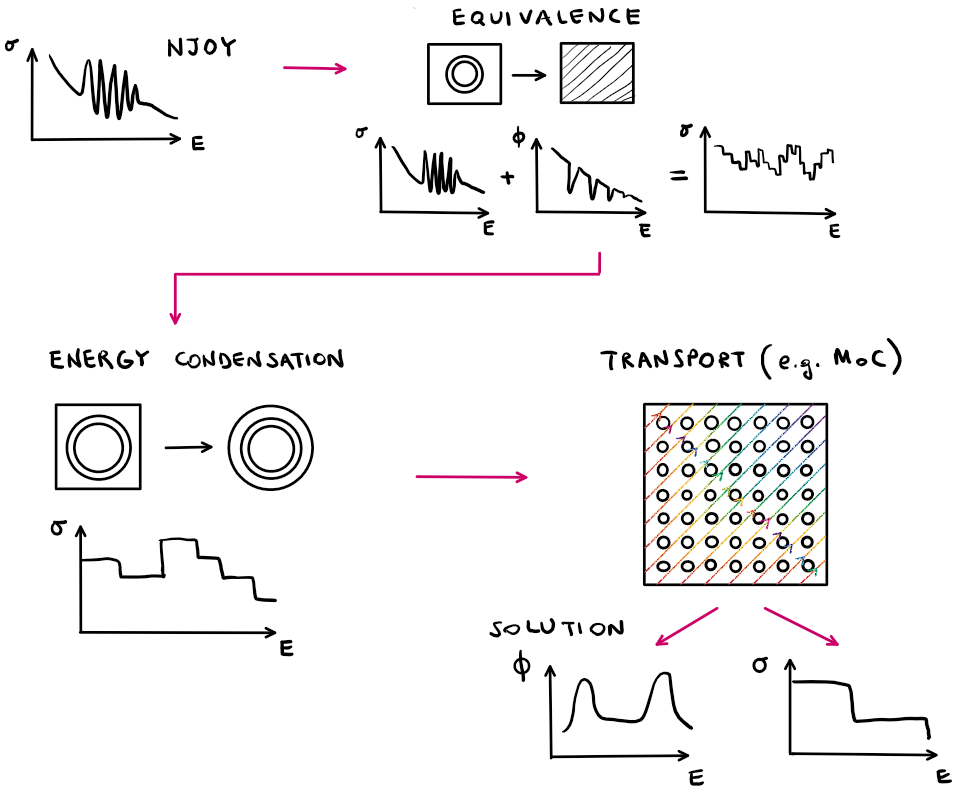
\includegraphics[scale=0.60]{./images/summary_lattice_physics.png} 
	\caption{The overall flow lattice physics calculations before homogenisation.} 
	\label{fig:lattice_physics}
\end{figure}

\section{Energy condensation}

From having fine-group (100s of groups) MG cross sections, we want to obtain few-group (typically dozens of groups) MG cross sections in preparation for a fine-mesh transport calculation across the problem. This requires generating unique flux spectra in each material region of our problem (typically a 2D assembly or several assemblies). The more accurate the spectrum generated at this stage, the fewer groups we can get away with having during fine-mesh transport calculations. In principle we could go directly to fine-mesh assembly-scale transport in 100s of groups but, as usual, that was historically too computationally expensive for most codes to do, especially when one must analyse many assemblies in different conditions during core design and reloading optimisation. 

Obtaining accurate spectra across each unique pin cell of course requires many fast transport calculations. The preferred means of doing this is by 1D collision probabilities calculations. While pins usually have square (or hexagonal) boundaries, they are `cylindricalised' because this allows the 1D calculation with analytic values of the probabilities to be used. This is shown in Fig.~\ref{fig:cylinder}. As an aside, this usually necessitates using `white' boundary conditions (neutrons are reflected back isotropically) rather than reflective or periodic boundaries. This is because in cylindrical geometries it is possible for reflected neutrons to never intersect the fuel, as also shown in Fig.~\ref{fig:cylinder}.

\begin{figure}[h!]
	\centering
	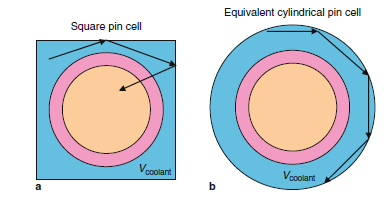
\includegraphics[scale=0.95]{./images/cylinder.png} 
	\caption{A regular pin cell, its equivalent cylinder version, and a demonstration of the effect of reflective boundaries on neutron streaming~\cite{Knott}.} 
	\label{fig:cylinder}
\end{figure}

To make these calculations even faster, they are often performed as fixed source calculations, i.e., a fission spectrum source is imposed directly on the boundary and in the fuel and therefore one needn't solve the problem as an eigenvalue problem (removing one layer of iteration). Imposing a fission spectrum at the boundary allows for generating accurate cross sections even in fuel pins which can't sustain fission, such as pins with burnable absorbers or water rods.

Once a spectrum has been produced in the energy structure of the code's nuclear data library, $\{g\}$, it is used to condense the cross sections into some given coarser group structure $\{G\}$. This is done as:
\begin{equation}
    \Sigma^G_{x,i}=\frac{\sum_{g\in G}\Sigma^g_{x,i}\phi^g_i}{\sum_{g\in G}\phi^g_i}\;\mathrm{,}
\end{equation}
where $x$ is any generic reaction and $i$ is an index for a given region of the problem.

Note in general \textbf{there is no known optimal coarse group structure!} Often this is determined simply by trial and error and/or user experience!

\section{Fine-mesh transport}

Following condensation, we proceed to obtain a fine-mesh transport solution across the whole assembly. This is invariably performed with MoC due to its ability to handle the exact geometry of an assembly lattice. As a reminder, a typical mesh discretisation for a standard PWR assembly is shown in Fig.~\ref{fig:disc} (as stolen from the Lecture 3 notes).

\begin{figure}[h!]
     \centering
    \begin{subfigure}[t]{0.45\textwidth}%
    \captionsetup{justification=centering}
         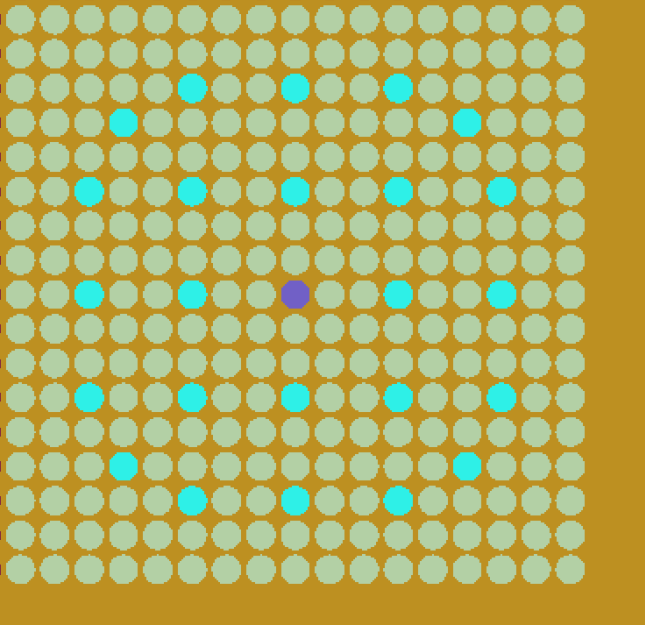
\includegraphics[scale=0.65]{./images/assembly.png}%
         \caption{A single PWR assembly surrounded by water}
         \label{fig:C5G7}
    \end{subfigure}
    \begin{subfigure}[t]{0.45\textwidth}
    \captionsetup{justification=centering}
         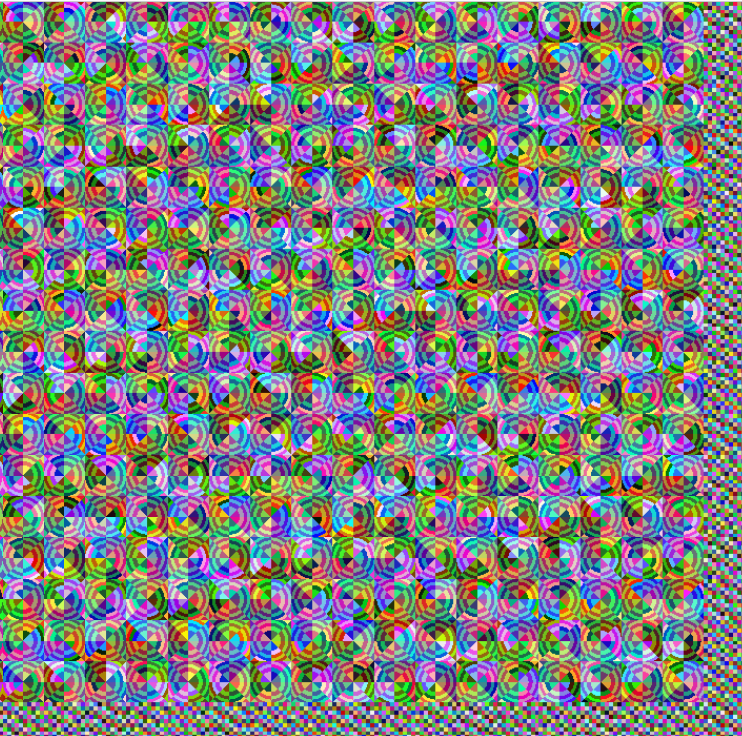
\includegraphics[scale=0.555]{./images/assembly_disc.png} 
	       \caption{The discretisation of the assembly in standard calculations} 
	       \label{fig:MGMC_cells}
    \end{subfigure}
  
    \caption{MoC geometry and its discretisation}
    \label{fig:disc}
\end{figure}

This calculation is performed for several reasons. First, it accounts for the flux tilts and influences that may occur across an assembly, e.g., the influence of unlike pins, burnable absorbers, water rods, or control rods/blades. Second, it allows for obtaining reaction rates which may be used to perform burn-up. Finally, with spatial effects resolved, it allows us to perform the final condensation and homogenisation step: producing a set of few-group cross sections that represent the entire assembly and can be used by fast-running nodal codes. This involves integrating over energy and the space of the entire assembly:
\begin{equation}
    \Sigma^G_x = \frac{\sum_i V_i \sum_{g\in G}\Sigma^g_{x,i}\phi^g_i}{\sum_i V_i \sum_{g\in G}\phi^g_i}\;\mathrm{.}
\end{equation}
More on all of that next lecture!

\section{Burn-up}

We obviously want to know how a reactor will perform as it burns up. Therefore, as well as obtaining transport solutions and generating assembly-wise few-group cross sections at a single point in time, we also want to do so for multiple burn-up points in the future.

Subject to a neutron flux, the evolution of nuclide $i$'s nuclide density, $N_i$, is given by the Bateman equation (no relation to Bateman street):
\begin{equation}\label{eq:bateman}
    \frac{\mathrm{d}N_i}{\mathrm{d}t} = \sum_j \gamma_{j\rightarrow i}\sigma_{\mathrm{f},j}\phi N_j + \sigma_{\mathrm{c},j\rightarrow i}\phi N_j +\lambda_{j\rightarrow i}N_j - \lambda_i N_i - \sigma_{\mathrm{a},i}\phi N_i\;\mathrm{,}
\end{equation}
where $t$ is time, $\gamma_{j\rightarrow i}$ is the fission yield of nuclide $i$ from fissioning $j$, $\sigma_{\mathrm{f},j}$ is the microscopic fission cross section of nuclide $j$, $\phi$ is the local scalar neutron flux, $N_j$ is the nuclide density of nuclide $j$, $\sigma_{\mathrm{c},j\rightarrow i}$ is the microscopic capture cross section of nuclide $j$ that results in the production of nuclide $i$, $\lambda_{j\rightarrow i}$ is the partial decay constant of $j$ to produce $i$, $\lambda_i$ is the decay constant of $i$, and $\sigma_{\mathrm{a},i}$ is the microscopic absorption cross section of $i$. As you can see, the first three terms on the right are production rates which produce nuclide $i$ from other nuclides, while the last two terms are the loss terms of nuclide $i$. The decay constants are obtained from the basic nuclear data libraries, while one-group microscopic cross sections/reaction rates are obtained by condensing the multi-group cross sections/reaction rates used during transport. Remember: transport is an \textbf{eigenvalue problem} therefore \textbf{the scalar flux can be scaled arbitrarily}. If we want to correctly perform burn-up calculations, the flux/reaction rates must be scaled to give the correct power/fission rate at which the assembly is operating.

If we refer to $\mathbf{N}$ as the vector of all nuclide densities and $\mathcal{A}$ as the burn-up matrix populated by all the coefficients which multiply a nuclide density in Eq.~\eqref{eq:bateman}, then Eq.~\eqref{eq:bateman} can be rewritten more compactly as:
\begin{equation}
    \frac{\mathrm{d}\mathbf{N}}{\mathrm{d}t} = \mathcal{A}\mathbf{N}\;\mathrm{.}
\end{equation}
If the nuclide vector is ordered in terms of increasing mass number, the burn-up matrix looks like that shown in Fig.~\ref{fig:matrix} if one considers a system of 1606 nuclides (most lattice codes consider $<$300). Can you tell which parts of the matrix correspond to which reactions? 

\begin{figure}[h!]
	\centering
	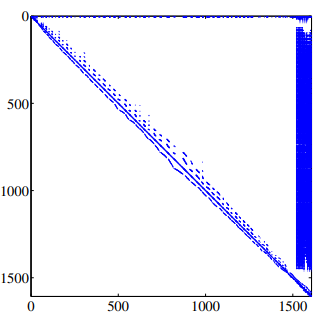
\includegraphics[scale=0.95]{./images/burnup_sparsity.png} 
	\caption{The sparsity pattern of a burn-up matrix containing 1606 nuclides \cite{Pusa}.} 
	\label{fig:matrix}
\end{figure}

This equation has the formal solution:
\begin{equation}
    \mathbf{N}(\Delta t) = \exp\left(\mathcal{A}\Delta t\right)\mathbf{N}(0)\;\mathrm{,}
\end{equation}
where $\Delta t$ is the time-step over which the problem is evolved, $\mathbf{N}(0)$ is the initial nuclide density vector, and $\exp\left(\mathcal{A}\Delta t\right)$ is known as a matrix exponential of $\mathcal{A}\Delta t$. For a matrix $\mathcal{B}$, the matrix exponential is defined in analogy with the regular exponential as:
\begin{equation}
    \exp\left(\mathcal{B}\right) = \mathbf{I} + \frac{\mathcal{B}}{1!} + \frac{\mathcal{B}^2}{2!} + \frac{\mathcal{B}^3}{3!}+\ldots\;\mathrm{,}
\end{equation}
where $\mathbf{I}$ is the identity matrix. Evaluating the matrix exponential is an extremely difficult numerical procedure -- there are famously many `dubious' ways to do so, and the best one is very problem dependent \cite{Moler}. Thankfully, there was once a PhD which showed that the Chebyshev Rational Approximation Method (often called CRAM) is a precise and numerically stable way to do it for burn-up problems. This is now the modern standard for solving burn-up problems. The actual operation requires a few (sparse) matrix inversions, but the justification requires quite a lot of complex analysis.

However, while it may be very possible to generate one-group microscopic cross sections at a single point in time, these will vary as burn-up proceeds due to changes in the spectrum. As such, one must either take short time-steps and then recalculate the cross sections, or one can use more sophisticated time-stepping algorithms which have a higher temporal order of accuracy. Unfortunately, this lecture has gone on too long already so this will have to be left for another time!

\printbibliography

\end{document}
